\chapter{Qualitätssicherung}
\label{chap:Qualitätssicherung}

Nach der erfolgreichen Implementierung des Übersetzers soll mit Hilfe einer zu testenden mobilen Anwendung überprüft werden,  ob der Compiler so arbeitet wie zu erwarten ist.  
\section{Testfälle}
Um die Anwendung vollständig Testen zu können, ist es notwendig Testfälle zu definieren anhand welcher die Soll-Situation mit der Ist-Situation verglichen werden kann.  Zu diesem Zweck werden in diesem Abschnitt Testfälle 

Tabelle \ref{tab:MetadataTests} zeigt die Testfälle für die Metadaten der mobilen Anwendung. 


\begin{table}[!ht]
\begin{tabularx}{\textwidth}{l|l|X}
   \textbf{Testfall-ID} & \textbf{Komponente} & \textbf{Beschreibung} \\
\hline
1             & App-Icon           	& Prüfen ob das App-Icon übernommen wurde                      			 \\ 
2             & App-Name          	& Prüfen ob das App-Name übernommen wurde                      		 \\ 
3             & SDK Versionen      & Prüfen ob die SDK Versionen übernommen wurden                      \\ 
\end{tabularx}
\caption{Testfälle für Metadaten}
 \label{tab:MetadataTests}
\end{table}

Tabelle \ref{tab:MenuTests} zeigt die Testfälle für die Navigation in der App. 


\begin{table}[!ht]
\begin{tabularx}{\textwidth}{l|l|X}
   \textbf{Testfall-ID} & \textbf{Komponente} & \textbf{Beschreibung} \\
\hline
1             & Seitenname           	& In der Navigationsleiste wird der Name der aktuellen Seite angezeigt                      			 \\ 
1             & Navigation         	& Mit Hilfe des Menüs kann navigiert werden                      			 \\ 
1             & Zurück Navigation           	& Über die Navigationsleiste kann zurrück Navigiert werden                      			 \\ 
\end{tabularx}
\caption{Testfälle für die Navigation}
 \label{tab:MenuTests}
\end{table}

Tabelle \ref{tab:Controls} zeigt die Testfälle für die Steuerelemente in der App. 

\begin{table}[!ht]
\begin{tabularx}{\textwidth}{l|l|X}
   \textbf{Testfall-ID} & \textbf{Komponente} & \textbf{Beschreibung} \\
\hline
1             & App-Icon           	& Prüfen ob das App-Icon übernommen wurde                      			 \\ 
\end{tabularx}
\caption{Testfälle für die Steuerelemente}
 \label{tab:Controls}
\end{table}

Tabelle \ref{tab:Sensoren} zeigt die Testfälle für die Verwendung von Sensoren in der App. 

\begin{table}[!ht]
\begin{tabularx}{\textwidth}{l|l|X}
   \textbf{Testfall-ID} & \textbf{Komponente} & \textbf{Beschreibung} \\
\hline
1             & App-Icon           	& Prüfen ob das App-Icon übernommen wurde                      			 \\ 
\end{tabularx}
\caption{Testfälle für Sensoren}
 \label{tab:Sensoren}
\end{table}


Tabelle \ref{tab:Images} zeigt die Testfälle für die Arbeit mit Bildern in der App. 

\begin{table}[!ht]
\begin{tabularx}{\textwidth}{l|l|X}
   \textbf{Testfall-ID} & \textbf{Komponente} & \textbf{Beschreibung} \\
\hline
1             & App-Icon           	& Prüfen ob das App-Icon übernommen wurde                      			 \\ 
\end{tabularx}
\caption{Testfälle für die Arbeit mit Bildern}
 \label{tab:Images}
\end{table}


Tabelle \ref{tab:Listview} zeigt die Testfälle für die Arbeit mit einer Listviews. 

\begin{table}[!ht]
\begin{tabularx}{\textwidth}{l|l|X}
   \textbf{Testfall-ID} & \textbf{Komponente} & \textbf{Beschreibung} \\
\hline
1             & App-Icon           	& Prüfen ob das App-Icon übernommen wurde                      			 \\ 
\end{tabularx}
\caption{Testfälle für die Arbeit mit Listviews}
 \label{tab:Listview}
\end{table}


Tabelle \ref{tab:Carousel} zeigt die Testfälle für die Arbeit mit einer CarouselViews. 


\begin{table}[!ht]
\begin{tabularx}{\textwidth}{l|l|X}
   \textbf{Testfall-ID} & \textbf{Komponente} & \textbf{Beschreibung} \\
\hline
1             & App-Icon           	& Prüfen ob das App-Icon übernommen wurde                      			 \\ 
\end{tabularx}
\caption{Testfälle für die Arbeit mit einer CarouselView}
 \label{tab:Carousel}
\end{table}



\section{Testobjekt}
Anhand dieser Testfälle kann anschließend ein Xamarin.Forms Projekt erstellt werden, anhand welcher der Source-To-Source Compiler getestet werden kann.  Im folgenden werden die Funktionalitäten der mobilen Anwendung dargelegt und mit Hilfe von iOS Screenshots dargestellt,  die entsprechenden Android Screenshots werden der Vollständigkeitsannahme in \nameref{chap:AnhangAndroidScreenshots} dargestellt. 

Bei der Anwendung sind in einem ersten Schritt die Metadaten der Anwendung relevant.  Dazu gehören der Name der Anwendung sowie das Anwendungsicon - außerdem sollten die SDK Version der mobilen Anwendung nicht modifiziert werden. Nach dem Start der Anwendung wird eine Menustruktur angezeigt,  über den verschiedene Bereiche der Anwendung angesteuert werden können.  In Abbildung \ref{fig:TestObjectI} werden Screenshots der mobilen Anwendung gezeigt.

\begin{figure}[!ht]
 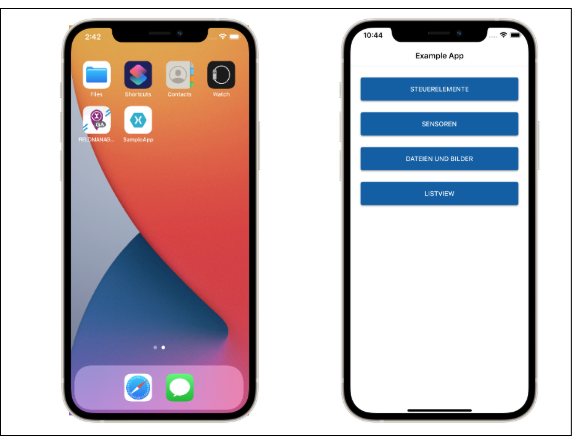
\includegraphics[width=\textwidth,keepaspectratio]{Images/Screenshot/AppIconAndMenu.png}
 \caption{Test Objekt Screenshots I}
 \label{fig:TestObjectI}
\end{figure}

Über dieses Menu kann der Anwender zu verschiedenen Seiten navigieren, die folgend kurz erläutert werden sollen.  Die in Abbildung \ref{fig:TestObjectII} zeigt die Seite mit den verfügbaren Steuerelementen von Xamarin.Forms,  wie sie auch in Kapitel 3 beschrieben wurden. Dazu gehören Ansichten für die Präsentation, für Interaktionen, zum setzen von Werten, für die Manipulation von Texten und für die Anzeige von aktuellen Interaktionen.
\begin{figure}[!ht]
 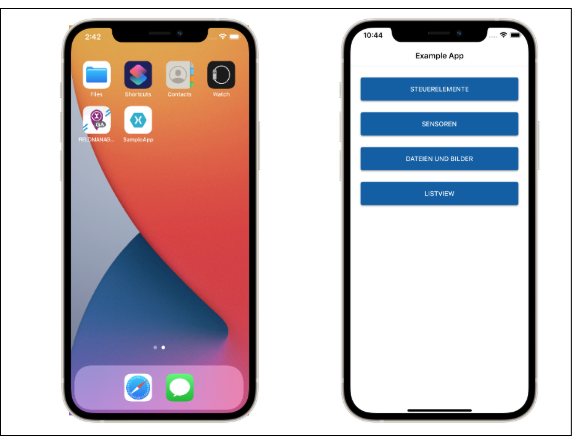
\includegraphics[width=\textwidth,keepaspectratio]{Images/Screenshot/AppIconAndMenu.png}
 \caption{Test Objekt Screenshots II}
 \label{fig:TestObjectII}
\end{figure}

Die folgende Option Sensoren öffnet eine Ansicht, auf der die aktuellen Werte von den Smartphone-Sensoren ausgegeben werden.  Diese Sensoren werden von vielen mobilen Anwendungen verwendet. Dazu gehören der Beschleunigungssensor, der Compass,  das Gyroscope und das Magnetometer.  Anhand dieser Seite,  soll sichergestellt werden, dass der Compiler auch die Funktionalität dieser Sensoren Abbilden kann. 

\begin{figure}[!ht]
 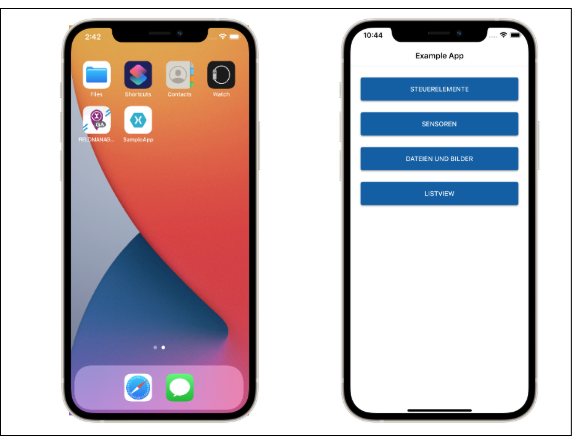
\includegraphics[width=\textwidth,keepaspectratio]{Images/Screenshot/AppIconAndMenu.png}
 \caption{Test Objekt Screenshots III}
 \label{fig:TestObjectI}
\end{figure}

Ebenfalls werden in dem Testprojekt eine Liste und ein Carousel abgebildet,  da es sich bei diesen um häufig verwendete Elemente handelt - die in vielen mobilen Anwendungen verwendet wird. 

\begin{figure}[!ht]
 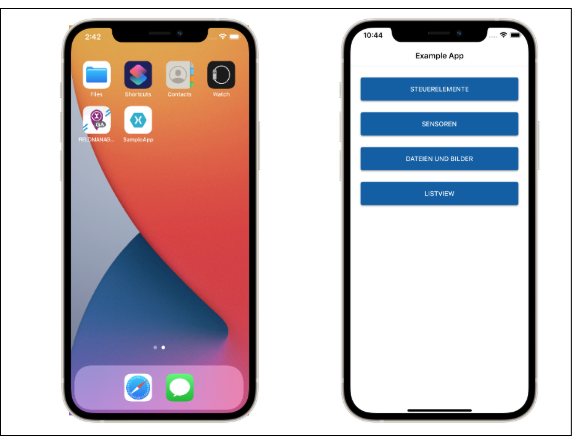
\includegraphics[width=\textwidth,keepaspectratio]{Images/Screenshot/AppIconAndMenu.png}
 \caption{Test Objekt Screenshots IV}
 \label{fig:TestObjectI}
\end{figure}




\section{Testablauf}




\section{Testauswertung}


